\documentclass[10pt]{article}

\usepackage{amsmath}
\usepackage{amssymb}
\usepackage{listings}
\usepackage{setspace}
\usepackage{color}
\usepackage[table]{xcolor}
\usepackage{hyperref}
\usepackage{pdflscape}
\usepackage{geometry}
\usepackage{tabu}
\usepackage{longtable}
\usepackage{graphicx}

\pagestyle{plain}

\setlength{\textwidth}{5.9truein}
\setlength{\textheight}{8.7truein}
\setlength{\oddsidemargin}{2.0mm}
\setlength{\evensidemargin}{2.0mm}
\setlength{\topmargin}{-20.5truemm}
\setlength{\parindent}{0.0truemm}
\parskip=1mm

\hypersetup{
	colorlinks=true,
	urlcolor=blue
}

\definecolor{lightgreen}{RGB}{149,240,149}

%Python colouring from http://widerin.org/blog/syntax-highlighting-for-python-scripts-in-latex-documents
\definecolor{Code}{rgb}{0,0,0}
\definecolor{Decorators}{rgb}{0.5,0.5,0.5}
\definecolor{Numbers}{rgb}{0.5,0,0}
\definecolor{MatchingBrackets}{rgb}{0.25,0.5,0.5}
\definecolor{Keywords}{rgb}{0,0,1}
\definecolor{self}{rgb}{0,0,0}
\definecolor{Strings}{rgb}{0,0.63,0}
\definecolor{Comments}{rgb}{0,0.63,1}
\definecolor{Backquotes}{rgb}{0,0,0}
\definecolor{Classname}{rgb}{0,0,0}
\definecolor{FunctionName}{rgb}{0,0,0}
\definecolor{Operators}{rgb}{0,0,0}
\definecolor{Background}{rgb}{0.98,0.98,0.98}

\lstset{
numbers=left,
numberstyle=\footnotesize,
numbersep=1em,
xleftmargin=1em,
framextopmargin=2em,
framexbottommargin=2em,
showspaces=false,
showtabs=false,
showstringspaces=false,
frame=l,
tabsize=4,
breaklines=true,
% Basic
basicstyle=\ttfamily\small\setstretch{1},
backgroundcolor=\color{Background},
language=Python,
% Comments
commentstyle=\color{Comments}\slshape,
% Strings
stringstyle=\color{Strings},
morecomment=[s][\color{Strings}]{"""}{"""},
morecomment=[s][\color{Strings}]{'''}{'''},
% keywords
morekeywords={import,from,class,def,for,while,if,is,in,elif,else,not,and,or,print,break,continue,return,True,False,None,access,as,,del,except,exec,finally,global,import,lambda,pass,print,raise,try,assert},
keywordstyle={\color{Keywords}\bfseries},
% additional keywords
morekeywords={[2]@invariant},
keywordstyle={[2]\color{Decorators}\slshape},
emph={self},
emphstyle={\color{self}\slshape},
%
}

\title{\bf DECO3801 Test Plan Document}
\author{\normalsize THEM - Typed HTML5 Evaluation Machine \\ \normalsize Carl Hattenfels, Scott Heiner, Shen Yong Lau, Robert Meyer, Brendan Miller, David Uebergang}

\date{}

\begin{document}

\maketitle

\section*{Functional Test Plan}

\subsection*{Testing Strategy}

There are three major testable components of our web application: the front-end website, back-end parser and database. While it was easy to write Python test cases for the back-end parser, it was more difficult to test our front-end website and database with a suite of computer-run tests. Instead, we wrote up a series of scenarios that we would undertake to ensure that the web application was running correctly and as expected. Clearly, all of these scenario tests can be ``implemented" as they are merely actions performed by us. This means that a test fails when some functionality is not yet implemented, or when fixing one error creates another error.

The test cases we are running on the parser can be found in Appendix A within this document. This gives an indication of the tests we have currently implemented in the system. More tests are being added periodically, as different types of HTML5 errors are added to the parser. Each HTML5 error will have its own associated test. Other parser related tests are also contained in Appendix A, including the JSON-RPC server tests. These test for concurrency (can the parser handle 5 concurrent requests?) as well as correctness of JSON-RPC input and output.

\subsection*{Implications of Functional Testing}

Our functional testing highlighted some issues with all aspects of our application. Primarily, there are several aspects of our functionality which are unimplemented at the moment but we hope to implement before the end of the project. However, we knew that these were issues. Instead, the interesting implications of the testing showed that we were mostly assured that we were programming our code correctly. We thought we had implemented an appropriate fix for the case of empty files (Website and Server Tests, 11) but our testing revealed this was an inadequate fix. Since we are still unsure of the implementation methods of each individual error check, many of the tests relating to errors are unimplemented. They will be periodically added as we introduce more error checks to the parser. From here, the next version of our prototype will aim to implement all the remaining functionality that our tests cover, and include tests on the remaining error parsing.

\newgeometry{margin=1cm}
\begin{landscape}
\pagestyle{empty}
\subsection*{Test Case Transcript}

{\bf Python Parser Tests}

\begin{center}
\begin{longtabu} to 10in {l | X<{\strut} | X<{\strut} | X<{\strut} | X<{\strut}}
Test Number & Test Description & Inputs  & Expected Output / Resulting Action & Pass / Fail + How to Fix \\
\hline
\hline
1
& Testing that a specific error is being reported correctly, given a particular fragment of HTML as the input. Since not all of the error checks have been or can be defined in advance, the implementation of this test case is reactionary and will be continually updated to include new error checks as they are added. The existing tests will have to be run each time a new error check is implemented to ensure that all existing functionality still works as intended. 
& A tailored fragment of HTML that should cause a specific error to be reported. eg. \texttt{``<head> <head> </head> </head>"} =\textgreater Testing for the duplicate set of head tags. & Confirmation that the expected error and associated error code is being returned for the given HTML fragment, in the expected character position of the input fragment.
& \cellcolor{lightgreen} Pass / Ongoing. The usage of this test case is currently being implemented after each error type is implemented. These tests are passing for the error checks we have implemented so far. \\
\hline
2
& Test that the JSON-RPC server is running and can respond to a remote function call.
& A single client making a function call to the server.
& The function call should be processed without an error being raised, implying the server is currently running.
& \cellcolor{lightgreen} Pass \\
\hline
3
& Testing that the JSON-RPC server is able to handle up to a maximum of 5 concurrent remote function calls.
& Five concurrent function calls are made to the server.
& The test case records the time that each response is received by each of the client instances. The function being called has an internal sleep delay of 2 seconds, so the recorded time for each client should be slightly over 2 seconds, implying all 5 calls were made and processed at the same time.
& \cellcolor{lightgreen} Pass \\
\hline
4
& Testing that a 6th concurrent connection (1 connection over the maximum of 5 concurrent connections) to the JSON-RPC server results in a delayed response.
& Six concurrent function calls are made to the server.
& As above, the time the response is received is compared to the time the call was made. The first 5 connections should behave as above, receiving a response in just over 2 seconds. The 6th call will receive a response after 4 seconds, 2 seconds after the server is able to respond after the first 5 connections have been responded to.
& \cellcolor{lightgreen} Pass \\
\hline
5
& Testing the parser's response to a case where input of an empty string is supplied.
& An empty string.
& The parser should respond with a general error stating that the input is empty, preventing other general errors such a missing closing HTML tags or page structure sections (head, body, footer).
& \cellcolor{pink} Failed. This check will have to be performed at the start of the main parsing loop, preventing the general structural errors from being reported. \\
\hline
6
& Testing the parser's response when the input string doesn't contain any valid HTML.
& A garbage string which doesn't contain any HTML tags or tag like elements eg. <blah>
& The parser should respond with a general error stating that the input doesn't contain any valid HTML.
& \cellcolor{pink} Failed. The parser will have to check the tokenizer for the existence of any valid tags. If none are found and the input string isn't empty, an error will be thrown stating that no valid HTML was found in the input. \\
\hline
7
& Testing that a correctly formed JSON-RPC 2.0 request is handled by the server, which should respond with the correct response.
& A JSON-RPC 2.0 request containing a small HTML code fragment to be parsed.
& A JSON-RPC 2.0 response containing an array of errors related to the given request. The response should also contain the same ID value as the one passed to it with the request.
& \cellcolor{lightgreen} Pass \\
\hline
8
& Testing that a malformed JSON-RPC 2.0 request containing incorrect parameters for a particular function call causes the server to return an error.
& A JSON-RPC 2.0 request containing an invalid parameters array for the function call \texttt{parse\_html}.
& A JSON-RPC 2.0 error response with a message of ``Invalid parameters".
& \cellcolor{lightgreen} Pass \\
\hline
9
& Testing that a JSON-RPC 2.0 request calling a function that isn't registered on the server causes the server to send an error response.
& A JSON-RPC 2.0 request containing a function name that hasn't been registered on the server.
& A JSON-RPC 2.0 error response with a message of ``".
& \cellcolor{lightgreen} Pass \\
\hline
10
& Testing the parser response when a tag with a URL attribute is supplied with an valid relative file path.
& Html fragment: \texttt{``<img src=``../image.jpg"><img src=``directory2/ image2.jpg">"}. File list: \texttt{[``image.jpg", ``directory/", ``directory/current.html", ``directory/directory2/ image2.jpg"]}. Current file: \texttt{``directory/current.html"}
& The parser response should NOT contain an error indicating an invalid file path.
& \cellcolor{lightgreen} Pass \\
\hline
11
& Testing the parser response when a tag with a URL attribute is supplied with an non-existent relative file path.
& Html fragment: \texttt{``<img src=../../image.jpg><img src=directory2/ image2.jpg>"}. File list: \texttt{[``directory/", ``directory/current.html"]}. Current file: \texttt{``directory/current.html"}
& The parser response should contain two errors indicating invalid file paths, associated with the src attributes of the img tags.
& \cellcolor{lightgreen} Pass \\
\hline
12
& Testing the parser response when a tag with a URL attribute is supplied with an non-existent files in existing relative filepaths.
& Html fragment: \texttt{``<img src=../image.jpg><img src=directory2/ image2.jpg>"}. File list: \texttt{[``directory/", ``directory/current.html", ``directory/directory2/"]}. Current file: \texttt{``directory/current.html"}
& The parser response should contain two errors indicating invalid file paths, associated with the src attributes of the img tags.
& \cellcolor{lightgreen} Pass \\
\hline
13
& Testing the parser response when a tag with a URL attribute is supplied with an valid absolute file path.
& Html fragment: \texttt{``<img src=/image.jpg><img src=/directory/directory2/ image2.jpg>"}. File list: \texttt{[``directory/", ``/image.jpg", ``directory/current.html", ``directory/directory2/", ``directory/directory2/ image2.jpg"]}. Current file: \texttt{``directory/current.html"}.
& The parser response should NOT contain an error indicating an invalid file path.
& \cellcolor{lightgreen} Pass \\
\hline
14
& Testing the parser response when a tag with a URL attribute is supplied with an non-existent absolute file path.
& Html fragment: \texttt{``<img src=/directory3/ image.jpg>"}. File list: \texttt{[``directory/", ``directory/current.html"]}. Current file: \texttt{``directory/current.html"}
& The parser response should contain an error indicating invalid file paths, associated with the src attributes of the img tag.
& \cellcolor{lightgreen} Pass \\
\hline
15
& Testing the parser response when a tag with a URL attribute is supplied with non-existent files in existing relative file paths.
& Html fragment: \texttt{``<img src=/directory/ image2.jpg>"}. File list: \texttt{[``directory/", ``directory/current.html"]}. Current file: \texttt{``directory/current.html"}.
& The parser response should contain one errors indicating invalid file paths, associated with the src attributes of the img tags.
& \cellcolor{lightgreen} Pass \\
\hline
\end{longtabu}
\end{center}

\newpage

\textbf{Website and Server Tests}

\begin{center}
\begin{longtabu} to 10in {l | X<{\strut} | X<{\strut} | X<{\strut} | X<{\strut}}
Test Number & Test Description & Inputs  & Expected Output / Resulting Action & Pass / Fail + How to Fix \\
\hline
\hline
1
& View Home page
& Go to URL, or click link from any page
& The home page is displayed.
& \cellcolor{lightgreen} Pass \\
\hline
2
& View Help page
& Click link from any page
& The user is sent to the help page.
& \cellcolor{lightgreen} Pass \\
\hline
3
& View Direct Input page
& Click link from any page
& The user is sent to the direct input page.
& \cellcolor{lightgreen} Pass \\
\hline
4
& Validate direct input
& The user types their input into the text field on the Direct Input page and clicks Validate.
& The input text is saved in a new set with a single file in it. The user is redirected to the Show File page.
& \cellcolor{lightgreen} Pass \\
\hline
5
& View Upload File(s) page
& Click link from any page
& The user is sent to the Upload File page.
& \cellcolor{lightgreen} Pass \\
\hline
6
& Upload single HTML file
& The user selects a file and then clicks Validate.
& The file is saved in a new set with a single file in it. The user is redirected to the Show File page.
& \cellcolor{lightgreen} Pass \\
\hline
7
& Upload multiple HTML files individually
& The user clicks the Add File button the required number of times, then selects a file for each field. They then click Validate.
& Files are saved in a new set, user is redirected to uploaded set page
& \cellcolor{lightgreen} Pass \\
\hline
8
& Upload multiple HTML files together from one dialogue
& The user selects multiple files in the dialogue box, then clicks Validate.
& Files are saved in a new set, user is redirected to uploaded set page
& \cellcolor{lightgreen} Pass \\
\hline
9
& Upload multiple HTML files, some individually and some from one dialogue box
& The user performs a combination of multiple Add Files and selecting multiple files in the dialogue boxes. They then click validate.
& Files are saved in a new set, user is redirected to uploaded set page
& \cellcolor{lightgreen} Pass \\
\hline
10
& Upload non-HTML file
& The user attempts to upload a file which is not HTML.
& The user is redirected to the same page and shown a information box informing them that the file chosen is not a HTML file.
& \cellcolor{pink} Failed. Currently it parses all uploaded files for HTML. Fix by checking mime type before sending to parser \\
\hline
11
& No file selected on upload
& The user attempts to upload a file when no file is selected.
& Redirect to upload file page with a helpful error message
& \cellcolor{pink} Failed. Currently an empty file is shown \\
\hline
12
& View Upload Zip page
& Click link from any page
& The user is sent to the Upload Zip page.
& \cellcolor{lightgreen} Pass \\
\hline
13
& Upload zip file
& Zip file selected on previous page, user clicked validate
& Zip archive is unpacked, files are saved in a new set, user is redirected to uploaded set page
& \cellcolor{lightgreen} Pass \\
\hline
14
& View Uploaded Set page
& User either uploads multiple files, or uploads a zip archive
& The user is shown the list of files uploaded in this set, with corresponding error bars.
& \cellcolor{lightgreen} Pass, except in the case of a single file in a set or zip, in which case the user is redirected directly to the show file page \\
\hline
15
& View Uploaded File page
& User either selects a file on the Uploaded Set page, or uploads a single file, or validates by direct input
& The user is shown their uploaded file, with corresponding error bar, general error information, and uploaded text with error highlighting.
& \cellcolor{lightgreen} Pass \\
\hline
16
& Remove file after certain period of being untouched in the server
& A file should be removed from the server after a period of inactivity.
& The files are removed from the database after a time. (3 hours)
& \cellcolor{pink} Failed. Currently, files stay in database. The cron job, which cleans up a file after it is left untouched for a time, is written and tested, but not installed on the development server \\
\hline
17
& User attempts to access files they have not uploaded
& The user manually attempts to alter the URL to view a file they have not uploaded.
& The user is redirected to the home page.
& \cellcolor{pink} Failed. Currently no security checking exists. The field exists in the data structure, but is not populated and validated against a php session id \\
\hline
\end{longtabu}
\end{center}
\end{landscape}
\restoregeometry
\pagestyle{plain}

\newpage

\section*{User Experience Goals}

We had a clear user experience in mind while developing this website. Through its ease of use and minimal effort on the part of the user, we have aimed to create a very surgical, ambient, and passive experience. The tool should give users almost immediate insight into the issues with their HTML and websites. This is where the user's experience with our tool ends, for this session. The user now can go and fix their file externally, return to our program and almost instantly receive another assessment of their code's validity. We do not aim to get the user invested in our system, and be held on the website for long periods at a time. However, we wish to create a reliable and worthwhile experience, brief as it is. The user should not be frustrated by the errors the program reveals, with the focus instead on \textbf{helping} the user learn and develop better web practices. It is meant to be a program that a user just ``touches", that is, they upload their file they want to check, and then go back and fix it, and then come back to this to validate again, in a cyclic process.

Our priorities are on quick and easy use, which is why all web pages are instantly accessible from all other web pages and users only need a few clicks to navigate. We have designed the website to require as few clicks as possible to access the primary functionality of the system. For example, the following images represent an average user's attempt to verify a file, after brief knowledge of the system's workings. \\

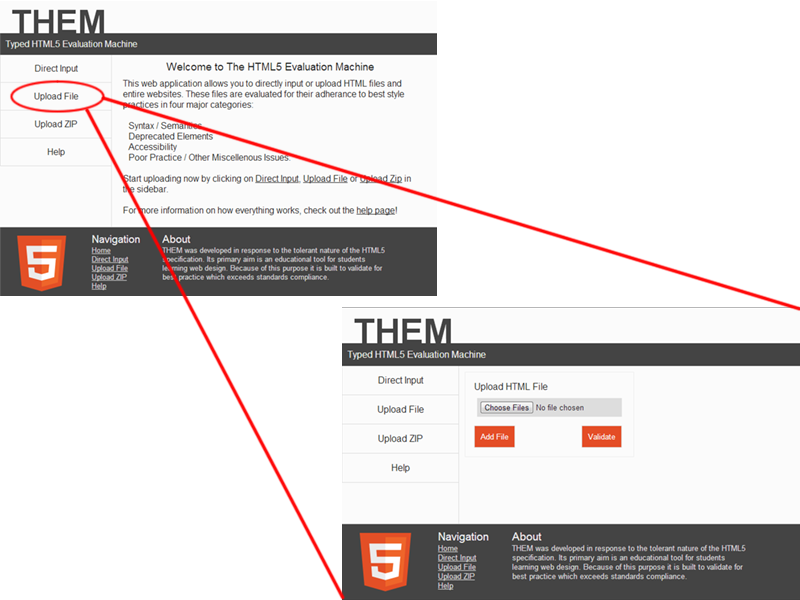
\includegraphics[scale=0.5]{click1.png}

The first click takes the user to the webpage.

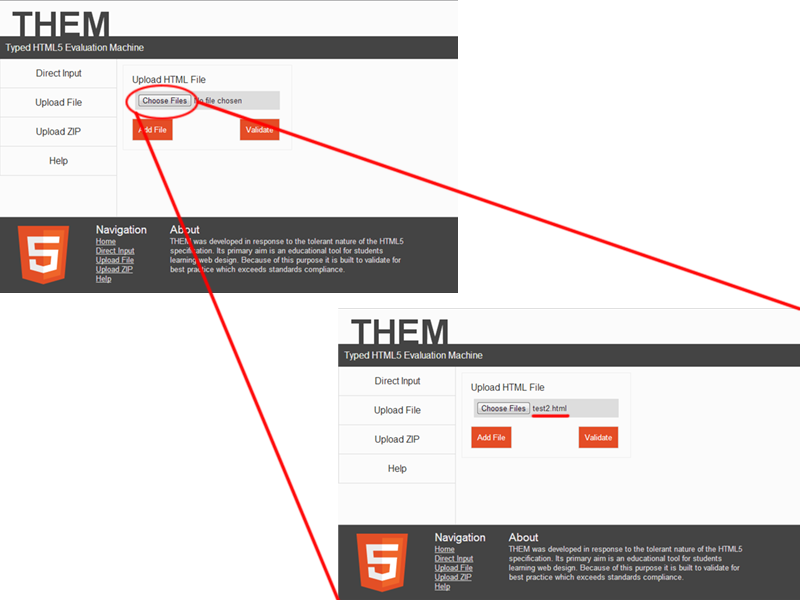
\includegraphics[scale=0.5]{click2.png}

The second click chooses a file to verify. Other clicks may be employed here as the user navigates their file system to find the file they want to upload.

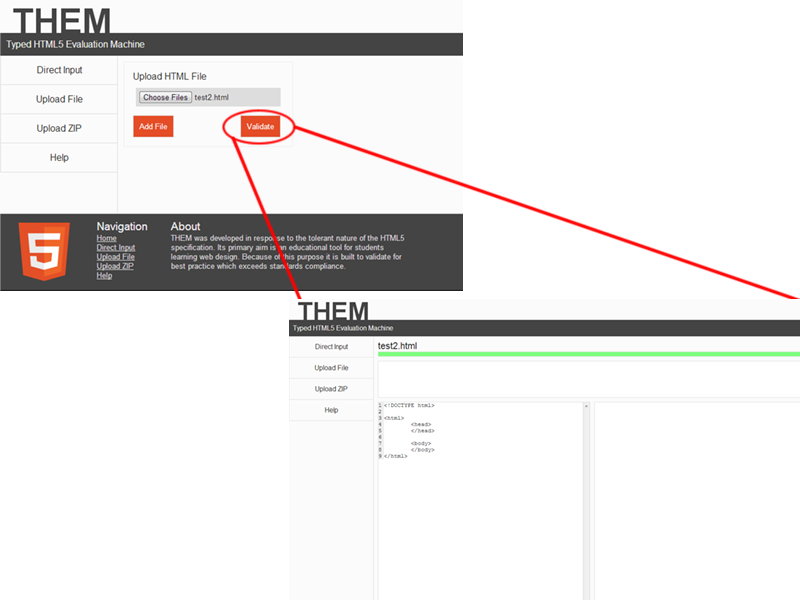
\includegraphics[scale=0.5]{click3.png}

The third click validates the selected file. In this way, the user quickly and easily travels from the opening page to viewing their validated HTML. All throughout the web application, we have aimed to create similar experiences where few clicks are required by the user, and they reach their end goal in minimal time.

\newpage

\section*{User Testing Plan}

\subsection*{User Testing Strategy}

Our web application will eventually be utilised by two user groups - students of DECO1400, and students of DECO7140. As such, we determined four major user testing groups:

\begin{itemize}
\item Undergraduate students who have already completed DECO1400
\item Undergraduate students who have not completed DECO1400 but have worked with computers
\item Masters students who have already completed DECO7140; and
\item Masters students who have not already completed DECO7140.
\end{itemize}

However, poor initial consideration due to this highly targeted user base caused us to primarily focus on students who had not done DECO1400, as these users represented students ``new" to DECO1400. Focusing also on past DECO1400 students would have allowed us to understand the needs of users who had previously completed the course, and could determine whether the tool would have been worthwhile to them. Poor communication on our part led to us getting very few in this category. Ultimately, we got information from nine users - four were undergraduates who had not done DECO1400, one was an undergraduate who had done DECO1400 and four were masters students who had done DECO7140.

We formulated six key scenarios for our users to undertake. Each scenario was performed on the live prototype at \underline{\url{http://underwaterfall.com}}. Storyboards for each of them can be found in the separately submitted Appendix B.

\begin{itemize}
\item Getting started by reading the help page (First Encounter Scenario) \\
\begin{tabular}{l p{3.5in}}
Actor: & New User \\
Goal: & To understand how the website works, and understand the feedback it provides. \\
Necessity of Scenario: & This scenario is required for first time users to understand how to use and interact with the program. \\
Preconditions: & User has not previously visited the webpage. \\
\end{tabular}
\item Validating HTML via Direct Input \\
\begin{tabular}{l p{3.5in}}
Actor: & User \\
Goal: & To check the validity of a piece of copied or typed HTML. \\
Necessity of Scenario: & This scenario represents one of the key ways users can get insight into how to program using HTML5. \\
Preconditions: & User has a clear understanding of the validation the website provides from the help page. \\
\end{tabular}
\item Validating HTML via uploading a file \\
\begin{tabular}{l p{3.5in}}
Actor: & User \\
Goal: & To check the validity of a HTML file. \\
Necessity of Scenario: & This scenario represents one of the key ways users can get insight into how to program using HTML5. \\
Preconditions: & User has a clear understanding of the validation the website provides from the help page. \\
\end{tabular}
\item Validating websites or multiple HTML files via uploading a zip \\
\begin{tabular}{l p{3.5in}}
Actor: & User \\
Goal: & To check the validity of a zip file of either website files or HTML. \\
Necessity of Scenario: & This scenario represents one of the key ways users can get insight into how to program using HTML5. \\
Preconditions: & User has a clear understanding of the validation the website provides from the help page. \\
\end{tabular}
\item Fixing a file based on the error suggestions, resubmitting and getting a valid file \\
\begin{tabular}{l p{3.5in}}
Actor: & User \\
Goal: & To check the validity of a piece of copied or typed HTML. \\
Necessity of Scenario: & This scenario is the primary point of the application - users learning to correct their HTML5 pages. \\
Preconditions: & User has already uploaded a file and determined the errors relating to their webpage. \\
\end{tabular}
\item Attempting to upload a non-HTML file (Fringe Case Scenario) \\
\begin{tabular}{l p{3.5in}}
Actor: & User \\
Goal: & To check the validity of a non-HTML file. \\
Necessity of Scenario: & Users are fallible and can upload incorrect files. They may also believe the website is capable of evaluating other types of files, like Javascript or CSS. \\
Preconditions: & N/A \\
\end{tabular}
\end{itemize}

We focused on the metrics of time taken to complete each scenario, and, in keeping with our surgical user experience, number of clicks required to complete each scenario. As we also wanted to create an enjoyable environment for the users, we also made note of any particular emotions and reactions of the users as they undertook the scenarios. Our primary strategy for user testing was as follows:

\begin{enumerate}
\item Prepare / lay out materials for the participant so that everything is ready.
\item Introduce ourselves to the participant and give them a high-level idea of what they will be doing in their tasks today.
\item Ask participant to fill in and sign consent form. The test conductor will fill in their parts too.
\item Give the participant more detailed instructions about the task they are to do (i.e. access the website, upload file and validate). Ask them to think out loud or to make comments as they work. See if there are any questions from the participants before we get started, and answer these where appropriate.
\item When participant is ready, ask the participant to start on the task. Start the timer. Be prepared to count the number of clicks they required to complete the task. Take hand notes as the participant works, according to the arrangements you have worked out amongst the non-participant group. If the participant goes a bit quiet, ask, ``what are you thinking now?" or ``what are you working on now?"
\item When they complete the first scenario, move them onto the next one, and so on.
\item After completing all six scenarios, ask the participant to fill in the questionnaire. Clarify as necessary.
\item When the participant has finished filling in the questionnaire, check over the responses to make sure that all parts have been filled out, and that the answers are legible.
\item Tell the participant that the session is at an end. Thank the participant for their time.
\end{enumerate}

You can see the results of testing below, after the ``Implications of User Testing" section, as well as the Questionnaire we used for testing.

\subsection*{Implications of User Testing}

In general, users had no trouble navigating the system. The average rating for how easy the system was to navigate was 4.78 / 5 on a Likert scale. We also clearly met our goal of the small number of clicks required for each operation. No user (from those who had click data registered) needed to click more than ten times. However, our system requires improvement in several key areas. On recommendation from the users, here is a key list of changes we plan to implement before the completion of this project:

\begin{itemize}
\item Invite the users to click on the error tags. Users often did not realise that they could click on the highlighted text to find out more about the error. We have already gone part way to completing this by changing the mouse from a text highlight symbol to a pointer finger commonly used with hyperlinks and buttons.
\item Errors with non-HTML files. As part of our user testing, we asked users to upload a non-HTML file, a common action which could be performed by a user. Many were surprised that the file was actually parsed. We plan to check the mimetype of the uploaded file, and prevent the parser from being passed non-HTML code. The user will be presented with an error on the Upload File screen when they attempt to upload a non-HTML file. The good news is that for the most part, the website did not break, except when a user attempted to upload a Powerpoint file. This should be prevented by the previously mentioned fix.
\item Add multiple files via Add File button. Users noted that an attempt to add a second file via the Add File button after selecting the first file caused their previously selected file to be forgotten. This needs to be fixed. One user had trouble due to the similarity of the Validate and Add File buttons, and we may look into making these two differ. However, as we have already implemented selecting multiple files from the file explorer itself, we may simply regress to this option, and discussion with our client may be necessary in this regard.
\item Blank file uploading. Users choosing no file in a file field of the form, along with some file fields being filled, were parsed as if they were files with no name. As such, they were sent to a set page showing bars with blank file names and error bars. These files should not be parsed, and if a user clicks Validate with no file selected, they should be redirected back to the user page and asked to upload a file.
\end{itemize}

We do not plan on redefining any test plans, but for future testing, we will likely work closer together to complete it. The differences between our methods of testing was obvious, and it lead us to getting less data than we could have gotten.

All in all, we believe that our web application was well received, with many users who had experience with HTML5 stating they would find our tool beneficial to their studies. We receiving a rating 4.6 / 5 on the Likert scale for ``How likely would you use this tool to assist you in your study?" among those students who had previous experience with HTML5. Although the tool still requires a lot of work to reach completion, it is well on the way to being a fantastic tool for users to evaluate their HTML5.

\newgeometry{margin=1cm}
\begin{landscape}
\pagestyle{empty}
\subsection*{User Test Results}

\textbf{Metric Results}

\begin{center}
\begin{longtabu} to 10in {l|l|X<{\strut}|X<{\strut}|X<{\strut}|X<{\strut}|X<{\strut}}
~& Get Informed & Direct Input & Upload a File  & Fixing a File& Upload Zip  & Upload Non-HTML File  \\ \hline\hline
Tester 1 - DECO1400  & ~& ~& ~  & ~& ~   & ~ \\ \hline\hline
Time taken (secs)& ~& 49.03& 39.9   & 32.7 & 13.3& 6.03  \\ \hline
Clicks   & ~& ~& ~  & ~& ~   & ~ \\ \hline
Reaction & ~& Confused about the highlighting word, unsure it is clickable & Feel confused when add file buton cancel previous upload entry & Learn the error quickly, getting used to the system presentation & Feeling comfortable & Feeling surprised when the result is as expected  \\ \hline\hline
Tester 2 - DECO7140  & ~& ~& ~  & ~& ~   & ~ \\ \hline\hline
Time taken (secs)& ~& 56   & 22.3   & 27   & 11.2& 6.5   \\ \hline
Clicks   & ~& ~& ~  & ~& ~   & ~ \\ \hline
Reaction & ~& Unsure about what the error bar representing & Frustrated as keep mispressing add file instead of validate due to same colour button  & Learn the error quickly  & Feeling comfortable & Feeling surprised when the result is as expected  \\ \hline\hline
Tester 3 - DECO7140  & ~& ~& ~  & ~& ~   & ~ \\ \hline\hline
Time taken (secs)& ~& 43.5 & 19.2   & 23.3 & 9.9 & 6.9   \\ \hline
Clicks   & ~& ~& ~  & ~& ~   & ~ \\ \hline
Reaction & ~& Feeling unimpressed as the error is not validated correctly  & Feeling satisfied with the simple way to upload file   & Learn the error quickly and fixed it & Feeling comfortable & Feeling surprised when the result is as expected  \\ \hline\hline
Tester 4 - DECO7140  & ~& ~& ~  & ~& ~   & ~ \\ \hline\hline
Time taken (secs)& ~& 51.2 & 23.1   & 31.78& 11.67   & 8.3   \\ \hline
Clicks   & ~& ~& ~  & ~& ~   & ~ \\ \hline
Reaction & ~& Feeling that the presentation of errors is good  & Frustrating when trying to upload multiple file, the add file button cancel previous entry & Learn the error quickly, feeling good& Feeling comfortable & Feeling surprised when the result is as expected  \\ \hline\hline
Tester 5 - DECO7140  & ~& ~& ~  & ~& ~   & ~ \\ \hline\hline
Time taken (secs)& ~& 48.12& 17 & 20.1 & 10.8& 5.87  \\ \hline
Clicks   & ~& ~& ~  & ~& ~   & ~ \\ \hline
Reaction & ~& Unsure about the highlighting words are clickable& Feeling good as it is easy to upload single file   & Learn the error quickly  & Feeling comfortable & Feeling surprised when the result is as expected  \\ \hline\hline
\newpage
Tester 6 - Undergraduate & ~& ~& ~  & ~& ~   & ~ \\ \hline\hline
Time taken (secs)& 7& 11   & 24.8   & 10   & 8   & N/A   \\ \hline
Clicks:  & 1& 2& 6  & 5& 4   & 5 \\ \hline
Reaction & ~& Didn't realise you could click on errors & ~  & Multiple files added but no files given - still shows the bars   & ~   & Powerpoint file uploaded - ``max\_allowed\_packets" error given \\ \hline\hline
Tester 7 - Undergraduate & ~& ~& ~  & ~& ~   & ~ \\ \hline\hline
Time taken (secs)& 2& 45   & 29 & 20   & 18  & 20 \\ \hline
Clicks:  & 1& 5& 5  & 3& 5   & 5 \\ \hline
Reaction & ~& ~& ~  & ~& ~   & Note, inf file still was parsed.  \\ \hline\hline
Tester 8 - Undergraduate & ~& ~& ~  & ~& ~   & ~ \\ \hline\hline
Time taken (secs)& 2& 41   & 14.8   & 63   & 22  & 13\\
Clicks:  & 1& 3& 6  & 8& 7   & 5 \\ \hline
Reaction & ~& ~& ~  & Backtracked to copy files, didn't get to put in entire tag   & ~   & ~ \\ \hline\hline
Tester 9 - Undergraduate & ~& ~& ~  & ~& ~   & ~ \\ \hline\hline
Time taken (secs)& 2& 60   & 28 & 211  & 9   & 15\\ \hline
Clicks:  & 1& 5& 6  & 9& 4   & 3 \\ \hline
Reaction & ~& ~& Clicked add file accidentally  & Not intuitive to click highlighted text  & ~   & ~ \\
\end{longtabu}
\end{center}

\newpage

\textbf{Questionnaire}

\begin{center}
\begin{longtabu} to 10in {l | X<{\strut} | X<{\strut} | l | l | l | l | l | l | l | X[3]<{\strut}}
Tester & Q1 & Q2 & Q3 & Q4 & Q5 & Q6 & Q7 & Q8 & Q9 & Q10 \\
\hline
\hline
Tester 1 & Yes (DECO1400, Programming) & Yes (Java, Javascript, PHP, Python) & 4  & 5  & 4  & 3  & 5  & No  & Yes & If you upload a non-zip file to the upload zip no error message is shown. Selecting file then clicking add file clears previous additions. Upload invalid file to upload file (specifically provided zip) shows the file. Adding \texttt{``<!DOCTYPE html>."} (note full stop) causes errors to appear (raw output). Clicking add file then only uploading 1 file takes you to collections screen instead of the single file screen. Leaving uploads blank causes blank error bars to appear. \\
\hline
Tester 2 & Yes (DECO7140) & Yes (Python, Java, Actionscript)& 3  & 2  & 4  & 5  & 4  & No  & Yes & ~ \\
\hline
Tester 3 & Yes (DECO7140) & No  & 4  & 4  & 4  & 4  & 4  & Yes & Yes & ~ \\
\hline
Tester 4 & Yes (B InfTech)& Yes (Java, PHP, C$\sharp$, HTML5, CSS, Javascript, MYSQL, etc) & 5  & 4  & 4  & 3  & 5  & No  & No  & Confused about the ``upload" buttons. Color theme is nice. Single file -\textgreater upload file, multiple files -\textgreater zip it and upload. Highlight the code in the correction section will be more user friendly (Upload File). General instruction on the UI can be added. Maybe do more market research about existing validation tools. Line mumber is good to be placed in direct input. \\
\hline
Tester 5 & Yes (DECO7140) & Yes (Actionscript, Python)  & 3  & 5  & 4  & 5  & 5  & No  & No  & Simple \& clean layout, I would like if I could copy the text and paste the text again to modify it. \\
\hline
Tester 6 & No & Yes (Python)& 2  & 4  & 4  & 2  & 5  & Yes & Yes & ~ \\
\hline
Tester 7 & No & Yes (Python, Java, Matlab)  & 2  & 4  & 4  & 3  & 5  & Yes & No & No way to gauge the effects of the error based on the error message. Didn't initially realise you can click on highlighted text to see error notes nor which colours associated to errors (thought colour was gauging error intensity.) \\
\hline
Tester 8 & No & Yes (Python, Matlab)& 3  & 5  & 4  & 4  & 5  & Yes & No  & All good :) \\
\hline
Tester 9 & No (though did make website in primary school) & Yes (Python, Matlab)& 1  & 4  & 4  & 5  & 5  & Yes & Yes & It was fun. \\
\end{longtabu}
\end{center}
\end{landscape}
\restoregeometry
\pagestyle{plain}

\subsection*{User Test Document}
\begin{center}
$\underline{\hspace{5in}}$
\end{center}

\documentclass[11pt]{article}

\usepackage{amsmath}
\usepackage{amssymb}

\setlength{\textwidth}{5.7truein}
\setlength{\textheight}{8.7truein}
\setlength{\oddsidemargin}{3.0mm}
\setlength{\evensidemargin}{3.0mm}
\setlength{\topmargin}{-21.5truemm}
\setlength{\parindent}{0.0truemm}
\parskip=2mm

\title{\bf \huge Brief Resume}
\author{Scott Heiner}

\date{}

\begin{document}

\maketitle

\section*{User Information}

Name: $\underline{\hspace{6cm}}$
Program or Degree: $\underline{\hspace{6cm}}$

\section*{Scenarios}


\section*{Questionaire}

\begin{enumerate}
\item Have you taken DECO1400/DECO7140? If not, do you have any past learning experience in web design (such as HTML4, Javascript, etc). \\ $\square$ Yes $\square$ No \\ Past learning experience: $\underline{\hspace{4cm}}$
\item Do you have any programming background, if so what languages you have been using? \\ $\square$ Yes $\square$ No \\ Past learning experience: $\underline{\hspace{4cm}}$
\item How likely would you use this tool to assist you in your study? \\ 
\begin{center}
\begin{tabular}{c | c | c | c | c}
Very likely & ~ & ~ & ~ & Very unlikely \\
5 & 4 & 3 & 2 & 1
\end{tabular}
\end{center}
\item How visually appealing is the website to you? \\
\begin{center}
\begin{tabular}{c | c | c | c | c}
Very appealing & ~ & ~ & ~ & Not very appealing \\
5 & 4 & 3 & 2 & 1
\end{tabular}
\end{center}
\item How well did this tool meet your expectations? \\
\begin{center}
\begin{tabular}{c | c | c | c | c}
Met my expectations very well & ~ & ~ & ~ & Did not meet my expectations \\
5 & 4 & 3 & 2 & 1
\end{tabular}
\end{center}
\item Do you feel comfortable with the presentation of the error message(s)? \\
\begin{center}
\begin{tabular}{c | c | c | c | c}
Very comfortable & ~ & ~ & ~ & Not very comfortable \\
5 & 4 & 3 & 2 & 1
\end{tabular}
\end{center}
\item How easy did you find the tool to navigate?
\begin{center}
\begin{tabular}{c | c | c | c | c}
Very easy & ~ & ~ & ~ & Very difficult \\
5 & 4 & 3 & 2 & 1
\end{tabular}
\end{center}
\item Is this your first time using HTML5 in developing a website? \\ $\square$ Yes $\square$ No
\item Would you prefer the option to select multiple files at once (in the explorer window) when uploading? \\ $\square$ Yes $\square$ No
\item If you have any general feedback/suggestions, feel free to use the space below to tell us. \\ \\
\setlength{\unitlength}{1cm}
\begin{picture}(12,5)
\put(0,0){\framebox(12,5){}}
\end{picture}
\end{enumerate}

\end{document}

\newpage

\section*{Appendix A - Python Test Code}

\subsection*{Syntax Tests}

\lstinputlisting{C:/Users/Veritas/Documents/GitHub/deco3801-them/parser/html5-python/html5lib/deco3801-tests/test_syntax.py}

\newpage

\subsection*{Page Structure Tests}

\lstinputlisting{C:/Users/Veritas/Documents/GitHub/deco3801-them/parser/html5-python/html5lib/deco3801-tests/test_page_structure.py}

\newpage

\subsection*{JSON-RPC Server Tests}

\lstinputlisting{C:/Users/Veritas/Documents/GitHub/deco3801-them/parser/src/tests/test_json_rpc_server.py}

\end{document}